El proyecto se desarrolló bajo el nombre \lstinline{multipurpose-app}, y desde el principio se organizaron las carpetas de manera que cada sección del proyecto quedara clara y ordenada. Esto no solo ayuda a mantener todo estructurado, sino que también hace que implementar los distintos módulos sea mucho más sencillo y ágil.

\begin{figure}[H]
    \centering
    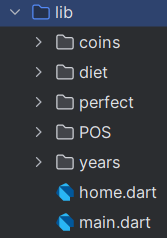
\includegraphics[width=0.4 \textwidth, height=5cm, keepaspectratio]{estructura_proy.png}
    \caption{Estructura de carpetas de proyecto}
    \label{fig:strpry}
\end{figure}

La navegación dentro de la app se maneja desde \lstinline{home.dart} usando una barra inferior, el \lstinline{NavigationBar}, que facilita moverse entre los distintos módulos. Para saber qué pantalla está activa en cada momento, se usa la variable \lstinline{currentPageIndex}. Cada vez que el usuario toca una de las pestañas, el método \lstinline{onDestinationSelected} actualiza ese índice, y gracias a eso el body del \lstinline{Scaffold} se encarga de mostrar dinámicamente el widget que corresponde a la sección seleccionada.

La interfaz también cuenta con una barra superior, o \lstinline{AppBar}, donde se muestra el título de la aplicación junto con algunos accesos rápidos. Al trabajar con un \lstinline{StatefulWidget}, cada módulo puede conservar su propio estado de manera independiente, lo que significa que las transiciones entre secciones son suaves y cada parte de la app funciona de forma autónoma sin interferir con las demás.
